\clearpage
\VerdierPhysicalPageAnchor{0141}%
\begingroup
\small
\setlength{\parskip}{0pt}%
\setlength{\emergencystretch}{1.5em}%
\setlength{\abovedisplayskip}{1pt plus 1pt minus 1pt}%
\setlength{\belowdisplayskip}{1pt plus 1pt minus 1pt}%

\VerdierSemanticAnchor{ch2-2-2-8-stepwise-conditions}
\noindent 使得：

\VerdierSemanticAnchor{ch2-2-2-8-condition-1}
\par\noindent\makebox[1.8em][l]{1)}$us_1=tu_1''$ 且 $s_1\in S$。
这是利用 SM2) 完成的。

\VerdierSemanticAnchor{ch2-2-2-8-condition-2}
\par\noindent\makebox[1.8em][l]{2)}$mQ(s_1s_2)=Q(f')$，其中
$f'\colon X_2''\longrightarrow X'$ 是 $\mathcal D$ 的态射，
$u_2''=u_1''s_2$，且 $s_2\in S$。这是利用定理 (2.2.2) 完成的。

\VerdierSemanticAnchor{ch2-2-2-8-condition-3}
\par\noindent\makebox[1.8em][l]{3)}$u'f's_3=gu_2''s_3$，
$u''=u_2''s_3$，且 $s_3\in S$。事实上，$\mathcal D$ 中的图式：

\VerdierSemanticAnchor{ch2-2-2-8-source-square}
\begin{center}
  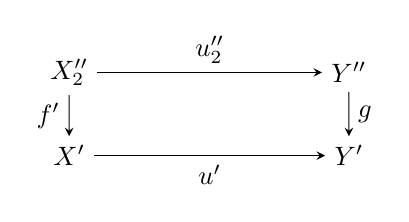
\begin{tikzpicture}[>=stealth,line width=.38pt,x=1.85cm,y=1.10cm,
    scale=.96,transform shape]
    \node (X2pp) at (0,1) {$X_2''$};
    \node (Ypp)  at (2,1) {$Y''$};
    \node (Xp)   at (0,0) {$X'$};
    \node (Yp)   at (2,0) {$Y'$};
    \draw[->] (X2pp) -- node[above] {$u_2''$} (Ypp);
    \draw[->] (X2pp) -- node[left] {$f'$} (Xp);
    \draw[->] (Ypp)  -- node[right] {$g$} (Yp);
    \draw[->] (Xp)   -- node[below] {$u'$} (Yp);
  \end{tikzpicture}
\end{center}

\VerdierSemanticAnchor{ch2-2-2-8-localized-commutativity}
\noindent 不一定交换。然而，对上述图式应用函子 $Q$ 所得的
$\mathcal D(S^{-1})$ 中的图式是交换的。因此有
$Q(u'f')=Q(gu_2'')\colon Q(X_2'')\longrightarrow Q(Y')$。

\VerdierSemanticAnchor{ch2-2-2-8-s3-refinement}
由 $\mathcal D(S^{-1})$ 中态射的定义，存在态射
$s_3\in S\colon X''\longrightarrow X_2''$，使
$u'f's_3=gu_2''s_3$。

\VerdierSemanticAnchor{ch2-2-2-8-proof-complete}
为完成引理的证明，只需令 $f=f's_3$，$s=s_1s_2s_3$。

\VerdierSemanticAnchor{ch2-2-2-9}
\smallskip
\noindent\textbf{2.2.9. 定理 2.2.6 证明的完成。}
\VerdierSemanticAnchor{ch2-2-2-9-triv-reduction}%
尚需证明集合 $T$ 具有性质 TRIV。现在已知该集合具有性质 TRI、TRII
与 TRIII。因此可以使用 1.2 的结果 (1.2.14)。特别地，由 (1.2.4)
可知，$T$ 中所有包含给定态射的三角彼此同构。于是，利用与命题
(1.3.2) 的证明中所用的归约类似的归约，对性质 TRIV 的证明可归结为
$\mathcal D(S^{-1})$ 中那些由 $\mathcal D$ 中的类似图式在 $Q$ 下的像
所得的图式。

\VerdierSemanticAnchor{ch2-2-2-9-reader-details}
此时验证是容易的。细节留给读者。

\VerdierSemanticAnchor{ch2-2-2-10}
\smallskip
\noindent\textbf{2.2.10.}\quad
设 $\mathcal D$ 为三角范畴，
$\mathcal B\subseteq\mathcal D$ 为满三角子范畴，$S(\mathcal B)$ 为
与 $\mathcal B$ 关联的乘法系 (2.1.15)。

\VerdierSemanticAnchor{ch2-2-2-10-quotient-category}
以 $\mathcal D/\mathcal B$ 表示范畴
$\mathcal D(S(\mathcal B)^{-1})$。范畴 $\mathcal D/\mathcal B$ 称为
\emph{$\mathcal D$ 关于 $\mathcal B$ 的商范畴}。

\VerdierSemanticAnchor{ch2-2-2-10-quotient-functor}
典范函子 $Q\colon\mathcal D\longrightarrow\mathcal D/\mathcal B$ 称为
\emph{商函子}。设 $F\colon\mathcal D\longrightarrow\mathcal D'$ 为到
某个三角范畴（分别地，阿贝尔范畴）的正合（分别地，上同调）函子。

\VerdierSemanticAnchor{ch2-2-2-10-kernel}
以 $\operatorname{Ker}(F)$ 表示由那些被 $F$ 送到零对象（分别地，
其所有平移都被 $F$ 送到零对象）的对象所定义的严格满且饱和的三角
子范畴，并称之为\emph{$F$ 的核}（(2.1.16) 与 (2.1.17)）。

\VerdierSemanticAnchor{ch2-2-2-10-p142-boundary}
\endgroup
